%\section{Software Implementation}
\section{Software Architecture} 
The crucial part of this project was to develop the firmware of the system. We choose the PlatformIO ecosystem and integrated it into Visual Studio Code. PlatformIO is an open-source ecosystem for IoT development that provides an IDE for various microcontroller platforms. 
\begin{figure}[htbp]
\centering
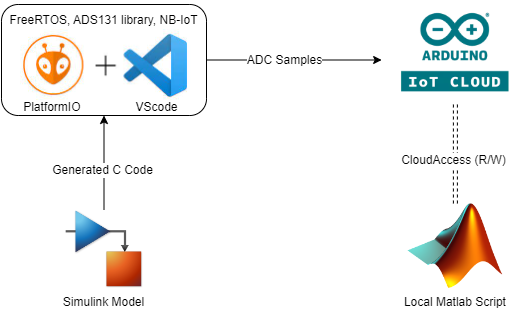
\includegraphics[scale=0.5]{images/Software Architecture.png}
\caption{Software Architecture}
\label{fig:x Software Architecture}
\end{figure}
The figure \ref{fig:x Software Architecture} depicts the whole software development process.We developed the ADC library within the firmware, along with configuring NB-IoT configuration within the Real-Time Operating System FreeRTOS. The ADC samples are transmitted to the Arduino Cloud, where the data can be read and written through a local Matlab script. Moreover, a Simulink model was created for computing RMS. This feature extraction algorithm generates C code that updates the firmware, enabling the calculation of subsequent samples within a synchronous function. Any kind of anomaly in electrical parameters are instantly available in cloud server.
\section{ADC Configuration \& Calibration} 
\subsection{Programming ADC} 
\textbf{Chip Select($\overline{CS}$):} The component is chosen to communicate by the active low input signal on the $\overline{CS}$ pin. When $\overline{CS}$ is set high, the device rejects all communication and DOUT has a high impedance. To assure excellent communication, we need to keep $\overline{CS}$ Low for the entire length of a communication period. Each time $\overline{CS}$ is taken high, the interface is reset. \par

\textbf{Serial Data Clock (SCLK):} The interface's serial clocking is provided through the input known as SCLK. The data that is input on DIN is latching onto the falling edge of SCLK, whereas the data output upon the DOUT pin transitions on the rising edge of SCLK. Our clock was tuned to 2.195MHz shown in figure \ref{fig:x Clock Generation}. \par
\begin{figure}[htbp]
\centering
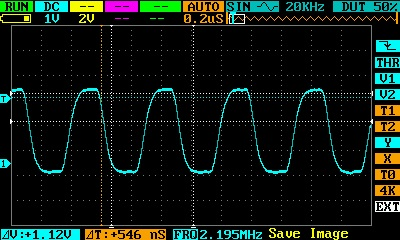
\includegraphics[scale=0.6]{images/2.195MHz.jpg}
\caption{Clock Generation for ADC}
\label{fig:x Clock Generation}
\end{figure}

\textbf{Serial Data Input (DIN):} Serial data entry for the device is performed employing the DIN pin. The device shifts a serial command in while the $\overline{CS}$ pin is low, via the DIN pin, for every SCLK falling edge. \par

\textbf{Serial Data Output (DOUT):} The device's DOUT pin acts as the serial data outputting pin. Whenever the $\overline{CS}$ pin is low, the device shifts out command responds and ADC data from conversion serially over each rising SCLK edge. Once $\overline{CS}$ is high, this pin approaches a condition of high impedance. \par

\textbf{Data Ready ($\overline{DRDY}$):} The $\overline{DRDY}$ pin represents an active low-powered output that signals while new conversions data are available in converting mode or whenever current detection criteria are satisfied in current-detect mode. \par

\textbf{SPI Communication:} Serial Peripheral Interface, is a widely used synchronous serial communication protocol that allows communication between microcontrollers, sensors, and other peripheral devices. The SPI communication typically involves one master device and one or more slave devices. The master device controls the communication by generating a clock signal (SCLK) and selecting the slave devices with a chip select signal ($\overline{CS}$). Each slave device has a unique $\overline{CS}$ pin to distinguish it from others on the bus.  \par
\vspace{1\baselineskip}\par 
Communication via the SPI with the ADS131M08 is carried out in frames. Each SPI signaling frame consists of multiple words. The word size may be set to 16 bits, 24 bits, or 32 bits through modifying the WLENGTH[1:0] bits in the MODE register.
\begin{figure}[htbp]
\centering
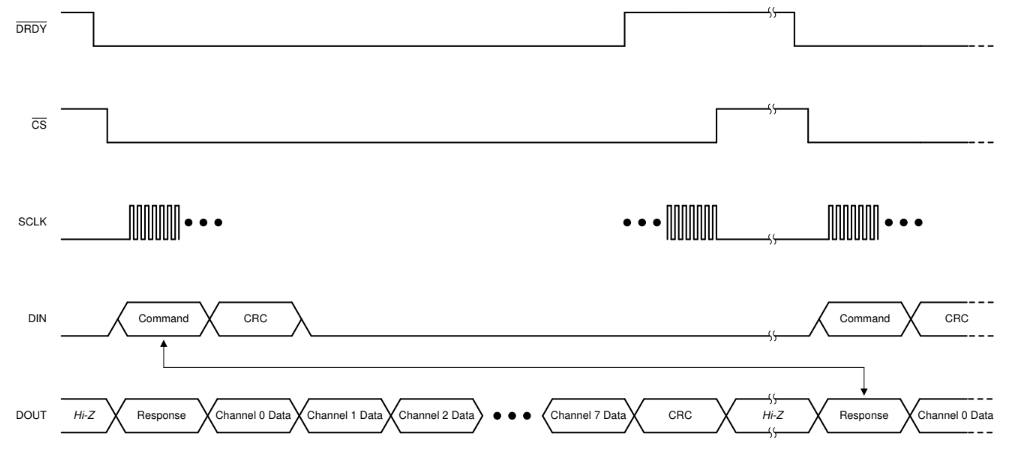
\includegraphics[scale=0.6]{images/Communication_Frame.png}
\caption{SPI Communication Frame}
\label{fig:x Communication Frame}
\end{figure}
The communication frame shown in figure \ref{fig:x Communication Frame} is full duplex, which means it can broadcast data on DOUT while receive data on DIN at the same time. The host's DIN input frames always starts with a single command. The answer to the command that was typed on the prior input frame is always the first word on the output frames that the system streams on DOUT. The amount of words in a command is determined by the command. A frame typically contains ten words for most instructions. The host supplies the command, the command CRC if inputs CRC is enabled, or one word of zeros if input CRC is disabled, and eight further words of zeroes on DIN. On DOUT, the unit concurrently produces the prior frames command's answer, eight words of ADC data denoting the eight ADC channels, and a CRC word.


\subsection{Setting Registers} 
\textbf{Register Map:} There are total 51 registers in ADS131M08. The details of each register's bit fields and their specific functions can be found in the device's datasheet \cite{ADSDatasheet}. Here we have presented all 51 registers name and address in Table \ref{tab:Register Map}. \par
\begin{table}[htbp]
  \centering
        \caption{Register Map of ADS131M08}
  \label{tab:Register Map}
  \adjustbox{width=1\textwidth, height=0.18\textheight}{
    \begin{tabular}{*{6}{|c}|}
      \hline
      \textbf{Address} & \textbf{Register} & \textbf{Address} & \textbf{Register} & \textbf{Address} & \textbf{Register} \\
      \hline
      00h   & ID   & 11h   & CH1\_GCAL\_MSB   & 22h   & CH5\_CFG  \\
      01h   & STATUS   & 12h   & CH1\_GCAL\_LSB & 23h   & CH5\_OCAL\_MSB    \\
      02h   & MODE   & 13h   & CH2\_CFG   & 24h   & CH5\_OCAL\_LSB   \\
      03h   & CLOCK   & 14h   & CH2\_OCAL\_MSB   & 25h   & CH5\_GCAL\_MSB    \\
      04h   & GAIN1   & 15h  & CH2\_OCAL\_LSB   & 26h   & CH5\_GCAL\_LSB   \\
      05h  & GAIN2   & 16h   & CH2\_GCAL\_MSB   & 27h   & CH6\_CFG    \\
      06h   & CFG   & 17h   & CH2\_GCAL\_LSB   & 28h   & CH6\_OCAL\_MSB     \\
      07h  & THRSHLD\_MSB   & 18h  & CH3\_CFG  & 29h   & CH6\_OCAL\_LSB \\
      08h   & THRSHLD\_LSB   & 19h   & CH3\_OCAL\_MSB   & 2Ah   & CH6\_GCAL\_MSB  \\
      09h   & CH0\_CFG   & 1Ah  & CH3\_OCAL\_LSB   & 2Bh   & CH6\_GCAL\_LSB   \\
      0Ah   & CH0\_OCAL\_MSB   & 1Bh   & CH3\_GCAL\_MSB  & 2Ch   & CH7\_CFG  \\
      0Bh   & CH0\_OCAL\_LSB   & 1Ch   & CH3\_GCAL\_LSB   & 2Dh   & CH7\_OCAL\_MSB  \\
      0Ch   & CH0\_GCAL\_MSB  & 1Dh   & CH4\_CFG  & 2Eh   & CH7\_OCAL\_LSB  \\
      0Dh   & CH0\_GCAL\_LSB   & 1Eh  & CH4\_OCAL\_MSB   & 2Fh   & CH7\_GCAL\_MSB \\
      0Eh   & CH1\_CFG   & 1Fh   & CH4\_OCAL\_LSB   & 30h   & CH7\_GCAL\_LSB   \\
      0Fh   & CH1\_OCAL\_MSB   & 20h   & CH4\_GCAL\_MSB   & 3Eh   & REGMAP\_CRC  \\
      10h   & CH1\_OCAL\_LSB  & 21h   & CH4\_GCAL\_LSB   & 3Fh   & RESERVED   \\
      % Add more rows here with additional elements...
      \hline
    \end{tabular}

  }

\end{table}

\subsection{Reading Registers} 
Configuring the registers of the ADS131M08 entails defining several parameters that dictate the ADC's behavior and functionality. The ADS131M08 offers multiple interface modes including SPI, QSPI, and parallel interface. In our case, we have opted for SPI communication to facilitate both data reading and writing.Then we have configured the power mode, input ranges, PGA, sampling rate and filter settings in the CONFIG (CFG) register. Additionally, a register tables of value and address also has been developed for in future R/W operation. The table \ref{tab:CLOCK Register} illustrates the process of reading the CLOCK register, which designates 16 bits for distinct functions. Among these, Bit 0 and 1 are designated for PWR, Bits 2-4 for OSR settings, Bits 5-7 are RESERVED, and the range from Bit 8 to 15 corresponds to eight distinct channels that enable specific functions. 
\begin{table}[htbp]
  \centering
  \caption{CLOCK Register Setting}
  \label{tab:CLOCK Register}
  \adjustbox{width=1\textwidth, height=0.04\textheight}{
  \begin{tabular}{|c|c|c|c|c|c|c|c|c|c|c|}
    \hline
    \multirow{2}{*}{\textbf{Address}} & 
    \multirow{2}{*}{\textbf{Register}} & 
    \multirow{2}{*}{\textbf{Reset}} & \textbf{BIT 15} & \textbf{BIT 14} & \textbf{BIT 13} & \textbf{BIT 12} & \textbf{BIT 11} & \textbf{BIT 10} & \textbf{BIT 9} & \textbf{BIT 8} \\
    \cline{4-11}
     & & & \textbf{BIT 7} & \textbf{BIT 6} & \textbf{BIT 5} & \textbf{BIT 4} & \textbf{BIT 3} & \textbf{BIT 2} & \textbf{BIT 1} & \textbf{BIT 0} \\
    \hline
    \multirow{2}{*}{03h} & 
    \multirow{2}{*}{CLOCK} & 
    \multirow{2}{*}{FF0Eh} & CH7\_EN & CH6\_EN & CH5\_EN & CH4\_EN & CH3\_EN & CH2\_EN & CH1\_EN & CH0\_EN\\
    \cline{4-11}
     & & & RESERVED & RESERVED  & RESERVED  & OSR[2] & OSR[1] & OSR[0] & PWR[1] & PWR[0] \\
    \hline
  \end{tabular}
}
\end{table}
For PWR we configured 00b(Very Low Power), and the OSR setting was 011b (1024 - 1kSPS). Though later we have updated the OSR at 001b (256 - 4kSPS). Figure \ref{fig:x Reading Register} depicts a simple example of reading the registers.
\begin{figure}[htbp]
\centering
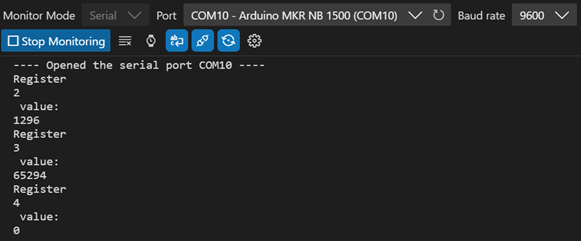
\includegraphics[scale=0.7]{images/Read_register.png}
\caption{Reading Register Values}
\label{fig:x Reading Register}
\end{figure}
\subsection{Reading Analog Data} 
 
\begin{figure}[htbp]
\centering
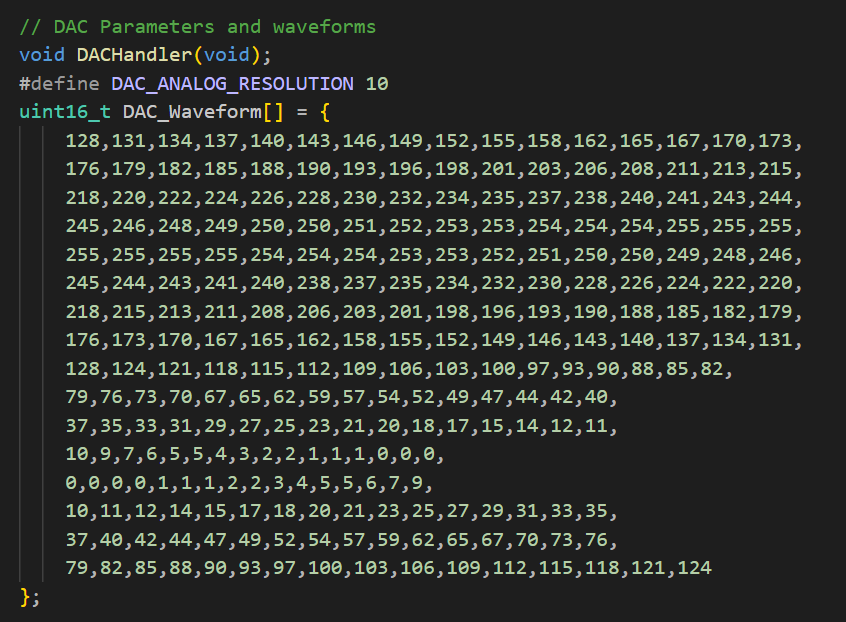
\includegraphics[scale=0.5]{images/DACWaveform.png}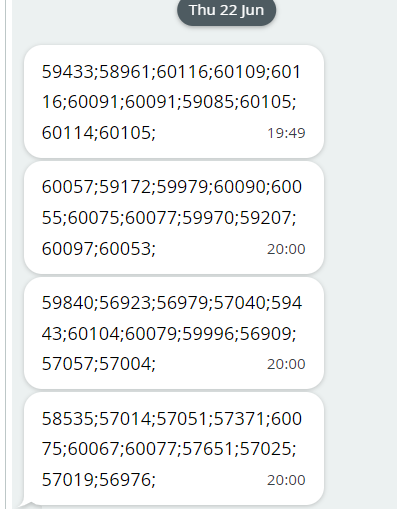
\includegraphics[scale=0.6]{images/SamplesCLOUD.png}
\caption{DAC Waveforms and Output}
\label{fig:x DAC_Waveforms}
\end{figure}
The process of generating an analog waveform using a Digital-to-Analog Converter (DAC) entails generating a sequence of digital values that align with the intended waveform.These digital values are then transmitted to the DAC to generate the corresponding analog signal. In our case, we generated a DAC waveform with a resolution of 10 bits and obtained the resulting output from the ADC, as depicted in the accompanying figure \ref{fig:x DAC_Waveforms}.
\section{Arduino IoT Cloud}
Arduino IoT Cloud serves as a platform facilitating seamless and secure connectivity between Arduino-based projects and the internet. It empowers the creation of IoT applications by simplifying the establishment of remote monitoring, control, and data collection for devices and sensors. The API Key tab grants access to essential credentials such as the client ID and secret keys, which are automatically generated upon thing creation. The ThingID is retrievable from the metadata section. Once the hardware integration with the cloud is finalized, it becomes possible to incorporate variables into things. These global variables are assigned specific IDs, enabling data reading and writing on the things using the Device ID, Thing ID, and Variable ID.
At initial attempt, we have to declare a total of four variables in our Arduino Cloud platform. These cloud variables name, type, operation, and ID has been listed in Table \ref{tab:Cloud variable} for a push button based data acquisition. Later, we have designed the variables and things to measure the RMS(I1,I2,I3), and RMS (V1,V2,V3), including Sync Period, and testing with NB-IoT. These variables dashboard has been shown in figure \ref{fig:x Cloud Variables}. 

\begin{table}[htbp]
  \centering
  \caption{Arduino Cloud variables for a single push button }
  \label{tab:Cloud variable}
   \adjustbox{width=1\textwidth, height=0.05\textheight}{
  \begin{tabular}{|c|c|c|c|}
    \hline
    \textbf{Cloud Variables} & \textbf{Variable Type} & \textbf{Variable Permission} & \textbf{Variable ID} \\
    \hline
    cloudADCParam  & Character string & Read \& Write & 58dd6174-6fe3-4173-9b38-154e90699878\\
    \hline
    cloudData  & Float  &  Read \& Write & 22a67deb-cf99-4950-8720-e62bff7a90cb \\
    \hline
    cloudPB  & Boolean & Read \& Write & 68d94ebb-f01e-4a8a-a799-41d945d9dbcf \\
    \hline
    cloudSamples  & Character string  & Read \& Write & f06b9506-f7c8-473a-af4c-8b4dd028d455  \\
    \hline
  \end{tabular}
  }
\end{table}

\begin{figure}[htbp]
\centering
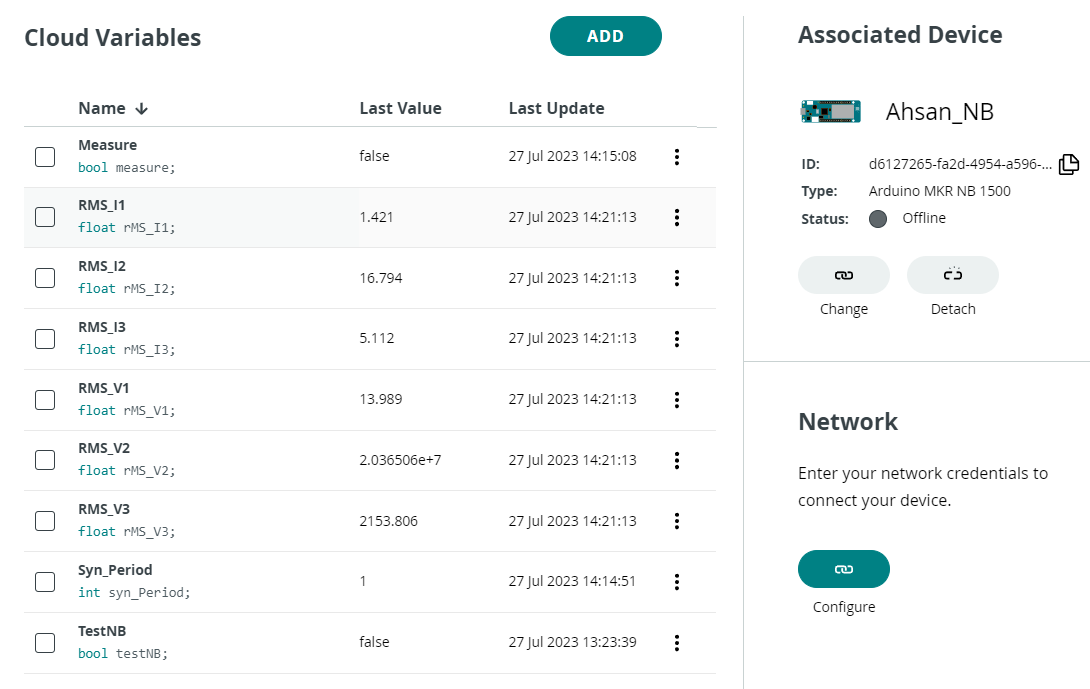
\includegraphics[scale=0.55]{images/Cloud Variables.PNG}
\caption{Cloud Variables for measuring RMS}
\label{fig:x Cloud Variables}
\end{figure}
In order to handle Arduino IoT Cloud Devices, Things, Properties, and Timeseries, the \href{https://www.arduino.cc/reference/en/iot/api/}{Arduino IoT Cloud API} offers a set of APIs. Any HTTP Client can be used to call this API. Also, Arduino Cloud provides a Web Editor which have a collection of code examples and libraries that we can use as a starting point for our IoT projects. This web editor helped us initially and running quickly without having to write code from scratch. The cloud dashboard offers a range of distinctive features that set it apart from other platforms. These include Data Visualization, widgets for easy configuration, a user-friendly Drag-and-Drop Interface, Real-Time Updates, the ability to set up Alerts and Notifications for multiple devices, and the flexibility for Customizations. These unique attributes played a significant role in our decision to select this platform for our project.

\section{Matlab WebAccess} 
\subsection{Data Reading and Writing}
To retrieve data from a web cloud using a MATLAB script, we can utilize various methods such as making HTTP requests, accessing APIs, or scraping web content. In the script of figure \ref{fig:x Matlab Response2}, the \textbf{‘webread’} function is used to make a \textbf{GET} request to the specified URL. The response from the API is a JSON object, which is then displayed in the MATLAB command window.\textbf{‘weboptions’} is a function in MATLAB that allows us to configure options for making HTTP requests using functions like webread or webwrite to interact with web services and APIs. It provides a way to customize various aspects of the request, such as headers, query parameters, timeouts, and more. This function is useful when we need to tailor the behavior of our HTTP requests to match the requirements of the web service we are interacting with.
The \textbf{‘strcat’} function in MATLAB is used to concatenate strings together. It takes multiple input arguments, which are strings or character arrays, and combines them into a single string.\par
\begin{figure}[htbp]
\centering
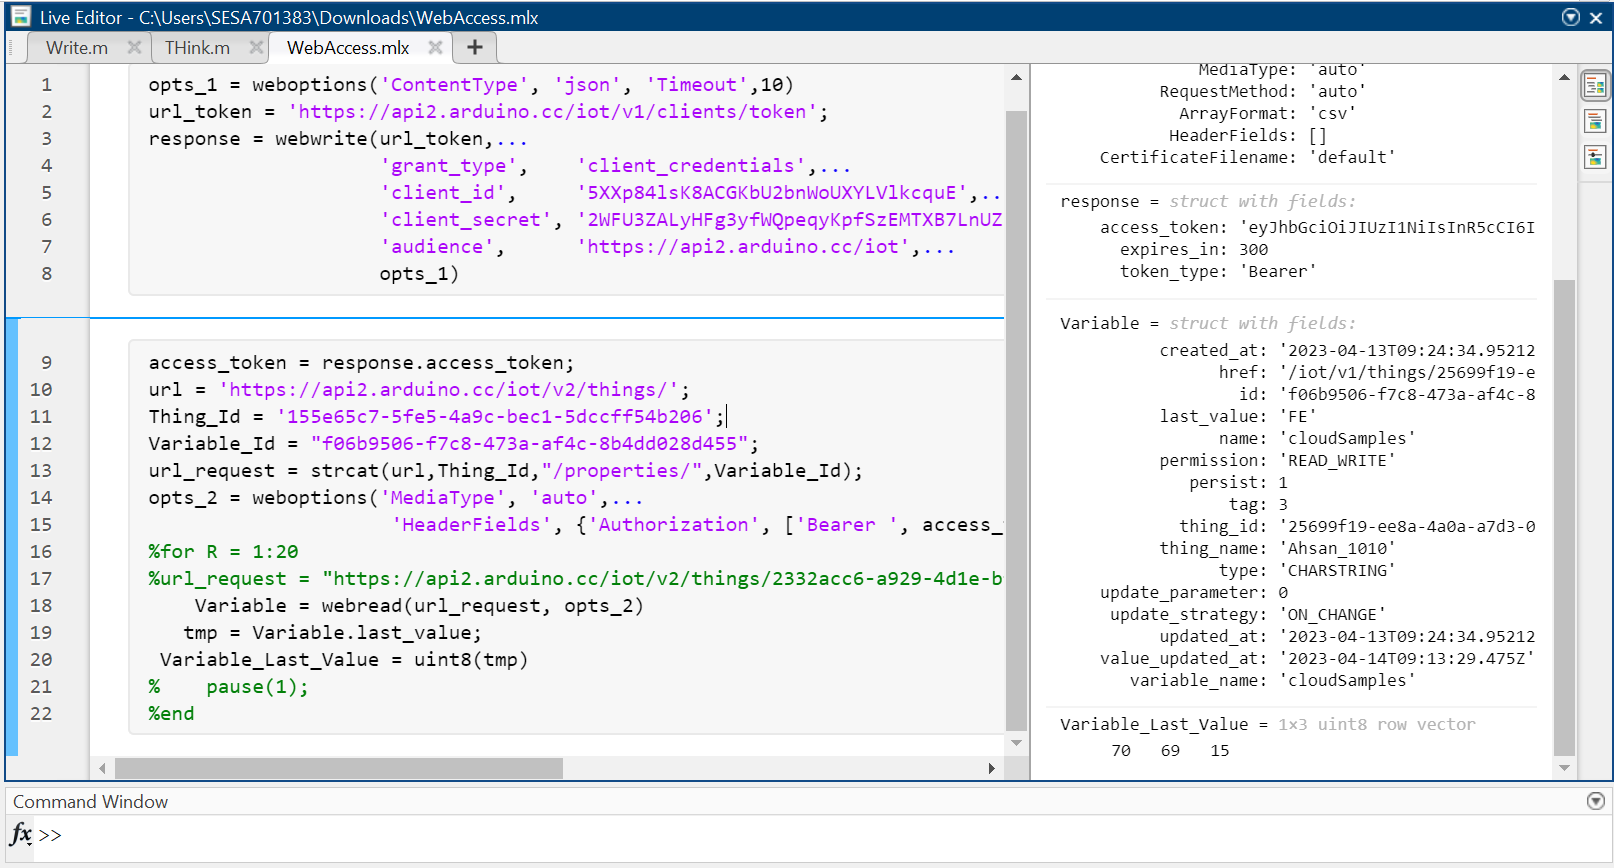
\includegraphics[scale=0.5]{images/Matlab Response2.PNG}
\caption{Data Reading from Cloud with Matlab}
\label{fig:x Matlab Response2}
\end{figure}
The \textbf{‘webwrite’} function in MATLAB is used to make HTTP \textbf{POST} requests and send data to a web service or API. It allows us to send data in various formats, such as JSON or form data, to a specified URL. Our data authentication process through MATLAB has few steps. At first, we need to get a authentication token which has been shown in the previous figure. Data reading from Arduino Cloud has been also depicted in previous figure. Then we write data to Arduino cloud variables by using webwrite, PUT command has been used in the weboption function. Finally, we have succeed to read historic data from the cloud and PUT the calculated unbalanced RMS values to the cloud variables demonstrated in figure \ref{fig:x Historical}.
\begin{figure}[htbp]
\centering
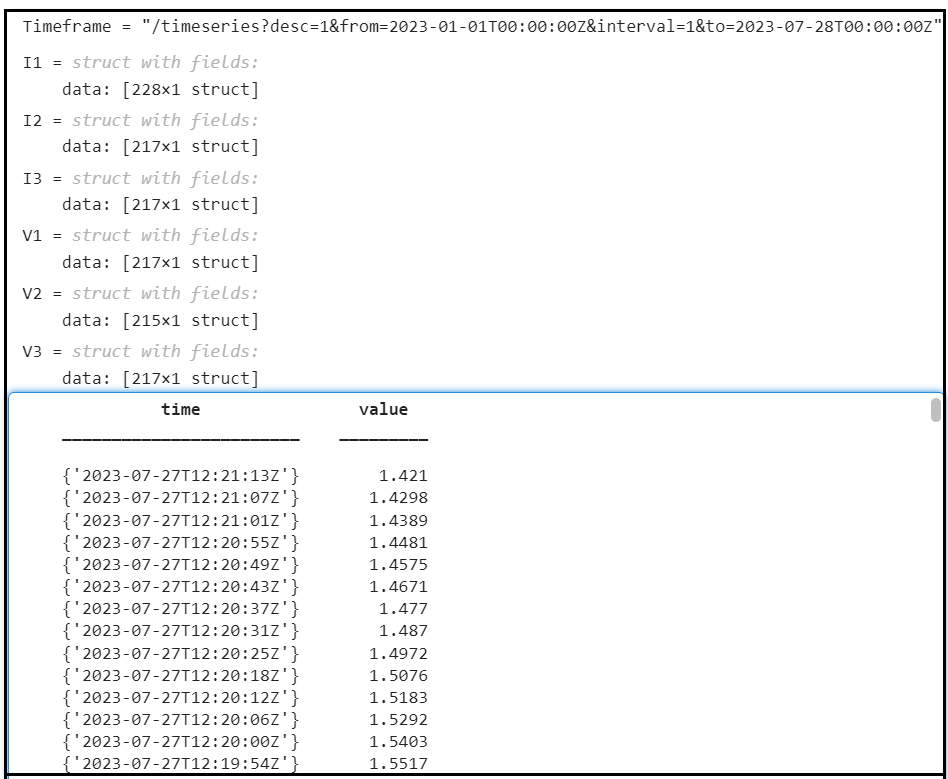
\includegraphics[scale=0.450]{images/HistoricData.PNG} 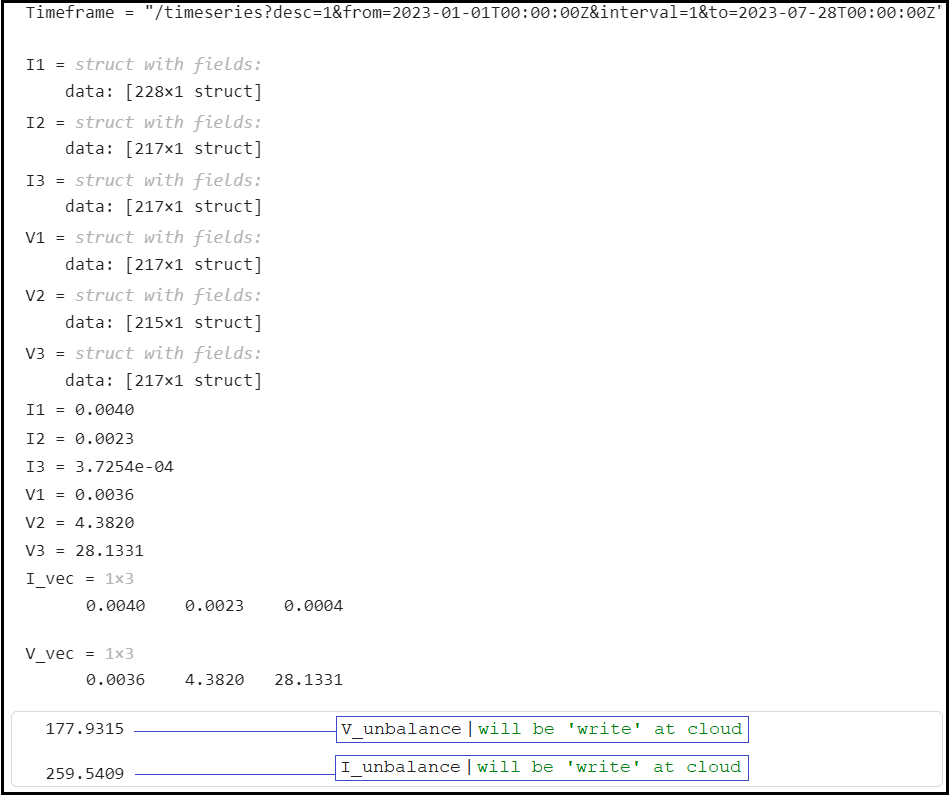
\includegraphics[scale=0.435]{images/UnbalancedWrite.PNG}
\caption{Historical data reading and writing unbalanced data}
\label{fig:x Historical}
\end{figure}
\subsection{Postman API}
During the MATLAB session we tested our API in \href{https://www.postman.com/}{Postman}. It allows us to create and send various types of HTTP requests, including GET, POST, PUT, DELETE, and more. We can specify request headers, parameters, body content, and authentication details. It supports various authentication methods, including basic authentication, API keys, OAuth 2.0, and more. We have used OAuth 2.0 authentication methos. Reading data from Arduino cloud by using GET API method has been demonstrated in figure \ref{fig:x Postman}.
\begin{figure}[htbp]
\centering
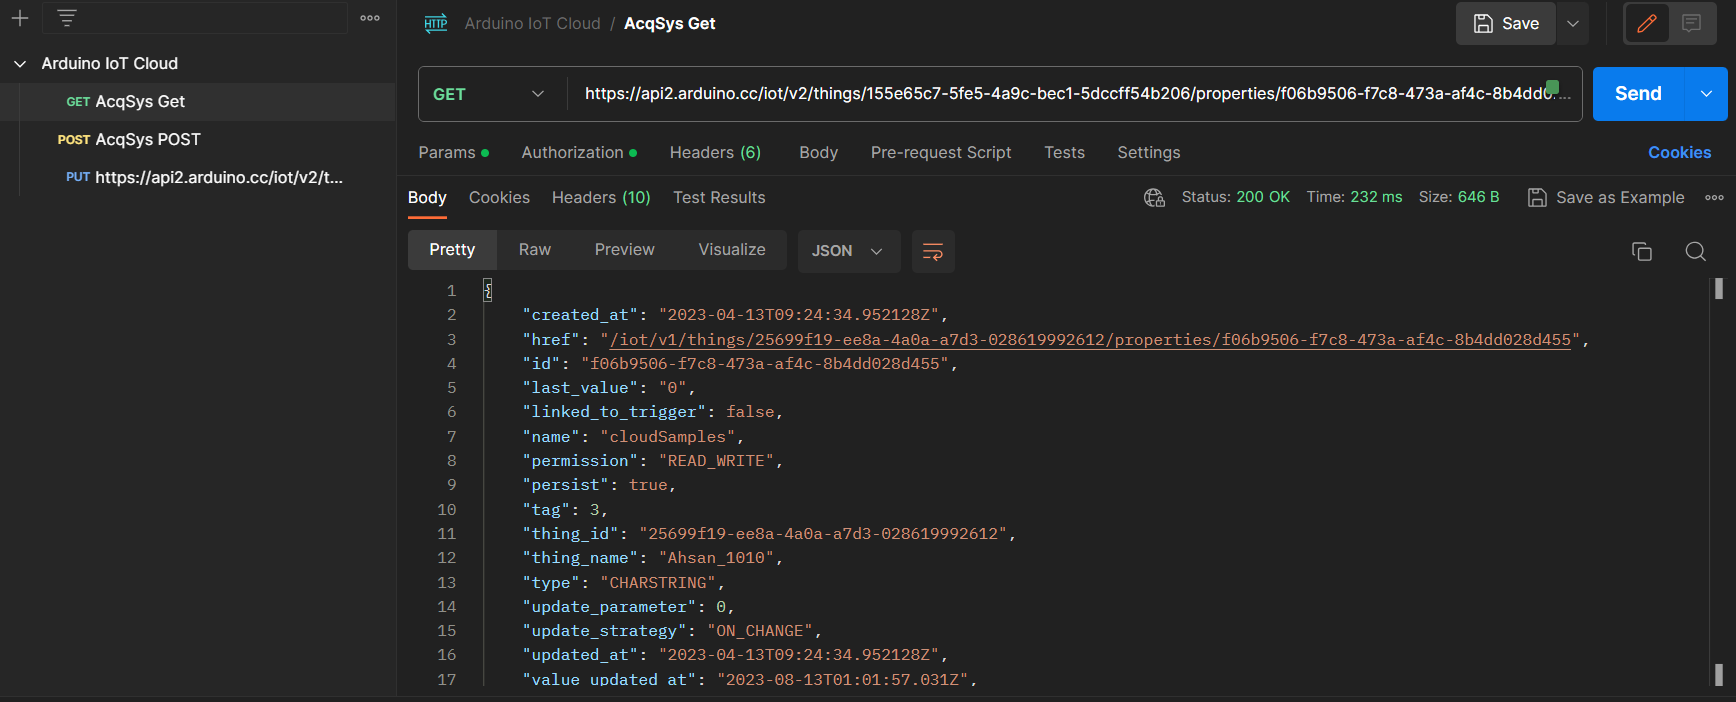
\includegraphics[scale=0.460]{images/postman.png} 
\caption{Configuring HTTP request through Postman API}
\label{fig:x Postman}
\end{figure}
\section{RTOS} 
\href{https://freertos.org/}{FreeRTOS} (Real-Time Operating System) is an open-source real-time operating system kernel for embedded systems. It provides a compact and efficient platform for developing applications that require precise timing and synchronization, making it well-suited for a wide range of embedded and IoT devices. FreeRTOS provides a manual for the mastering in Real Time Kernel included in \cite{FreeRTOS}. Also we studied another article to understand about FreeRTOS \cite{UnderstandingRTOS}. 

\subsection{Source files of FreeRTOS}
The fundamental FreeRTOS source code is present within only two C files that are universal across all FreeRTOS ports.  Tasks.c and List.c are both of them, and they can be found in the FreeRTOS/Source directory, as illustrated in Figure \ref{fig:x RTOS Tree}. 

\begin{figure}[htbp]
\centering
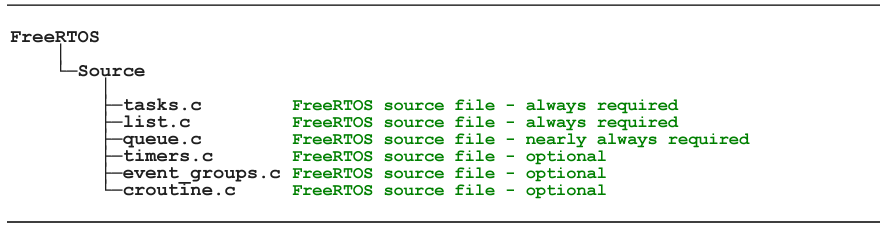
\includegraphics[scale=0.9]{images/FreeRTOS.png}
\caption{Core FreeRTOS source files in directory tree }
\label{fig:x RTOS Tree}
\end{figure}
The other source files also reside in the same directory as these two. The 3rd file from the source \textbf{‘queue.c’} provide a way for tasks to send and receive messages or data packets to/from each other in a thread-safe manner. It contains the implementation of the queue-related functions and data structures, including creating and deleting queues, sending and receiving data, blocking and unblocking tasks, and managing queue resources. Fourth one \textbf{‘timers.c’} provides the functionality for creating and managing software timers. Software timers are a key feature in FreeRTOS that allow tasks to be scheduled to run at specific intervals or after a certain delay, without the need for hardware timers. Fifth RTOS file from figure \textbf{‘event\_groups.c’} used for inter-task communication and synchronization in a multitasking environment. Event groups allow tasks to wait for specific combinations of events to occur. Tasks can set or clear individual bits within an event group, and other tasks can wait for a specific combination of bits to be set before continuing their execution. For the last one
\textbf{‘croutine.c’}, co-routines are a way to achieve cooperative multitasking within a single task context, allowing tasks to yield execution voluntarily to other tasks without relying on a preemptive scheduler. Co-routines are suitable for systems with limited resources, where full preemptive multitasking might be too heavyweight. They provide a mechanism for tasks to work together in a cooperative manner, sharing the CPU time based on their own scheduling decisions.\par
\vspace{0.5cm}\par
On the other hand, Heap management is an essential component for dynamic memory allocation required by tasks, queues, semaphores, and other kernel objects. Each task in FreeRTOS requires its own stack and potentially some heap space, depending on its memory requirements. In our firmware we used \textbf{‘heap\_4bis.c’}, which Implements thread-safe memory allocation using a critical section or mutex. It uses a block of memory provided by the application for the heap. The two main functions are \textbf{‘pvPortMalloc()’} and \textbf{‘pvPortFree()’}. These functions are used to dynamically allocate and deallocate memory from the heap.

\subsection{Header files of FreeRTOS}

A source file utilizing the FreeRTOS API should begin by including \textbf{‘FreeRTOS.h’}, followed by the appropriate header file housing the prototype for the utilized API function. These header files could be ‘task.h’,‘queue.h’,‘semphr.h’,‘timers.h’, or ‘event\_groups.h’. FreeRTOS.h is the main header file that we include in our OS. It provides access to the FreeRTOS API functions, data types, and macros. It also includes other necessary header files.
\textbf{‘task.h’} defines the functions and data structures for task management, creation, deletion, priority, and synchronization. queue.h provides the API for creating, using, and managing message queues. \textbf{‘semphr.h’} defines the API for creating and using semaphores for task synchronization and resource sharing. \textbf{‘event\_groups.h’} contains the API for creating and using event groups for inter-task communication and synchronization. \textbf{‘portmacro.h’} contains macros and functions that are specific to the architecture or port being used. This is where port-specific definitions and inline assembly might be defined. \textbf{‘FreeRTOSconfig.h’} contains architecture-specific or platform-specific configuration header files. These files allow us to configure various aspects of FreeRTOS behavior, such as tick rate, memory allocation scheme, and more. \textbf{‘croutine.h’} provides definitions and macros for co-routines, which are a lightweight form of multitasking. \textbf{‘portable.h’} has been included within a port layer's implementation to provide further port-specific definitions or macros.

\begin{figure}[htbp]
\centering
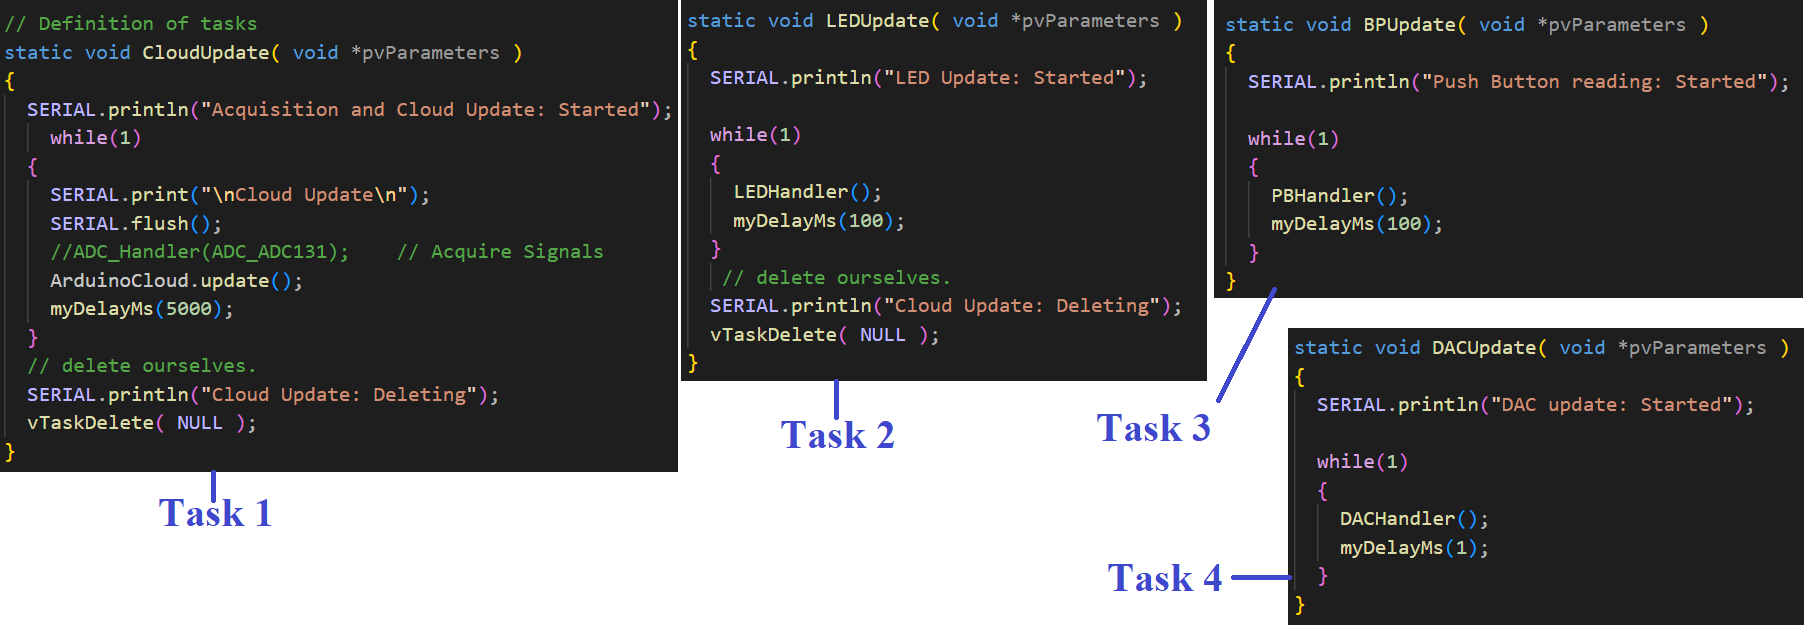
\includegraphics[scale=0.45]{images/Task1.png}
\caption{Task definition for acquisition system}
\label{fig:x RTOS Def}
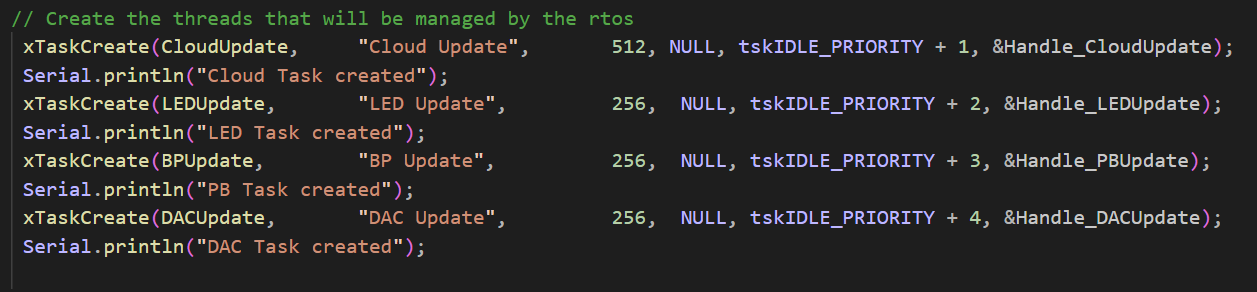
\includegraphics[scale=0.65]{images/RTOS_task.png} 
\caption{Scheduling the Tasks}
\label{fig:x RTOS Task}
\end{figure}
Task definition of our firmware has been depicted in the figure \ref{fig:x RTOS Def}, where we have created four different tasks CloudUpdate, LEDUpdate, BPUpdate, and DACUpdate. In figure \ref{fig:x RTOS Task}, all these four task scheduling has been depicted. Within this particular section, the task labeled Cloud Update commands a memory allocation of 512 bytes due to its elevated priority. Conversely, the remaining tasks have been assigned 256 bytes each, following a priority hierarchy where the sequence is as follows: LED Update $>$ BP Update $>$ DAC Update.


\section{Simulink Embedded Algorithm} 
Algorithms that are implemented on embedded systems, which are specialized hardware platforms made to carry out certain activities or operations, are referred to as embedded algorithms. Field-programmable gate arrays (FPGAs), microcontrollers, digital signal processors (DSPs), and application-specific integrated circuits (ASICs) are a few examples of hardware with limited computational resources that these algorithms are often made to operate efficiently on. To implement an algorithm in Simulink, a graphical representation of the algorithm's stages and calculations must be made. Simulink offers a visual platform for creating and modeling dynamic systems that incorporate methods from several fields, including signal processing, control systems, image processing, and more. 

\par
\begin{figure}[htbp]
\centering
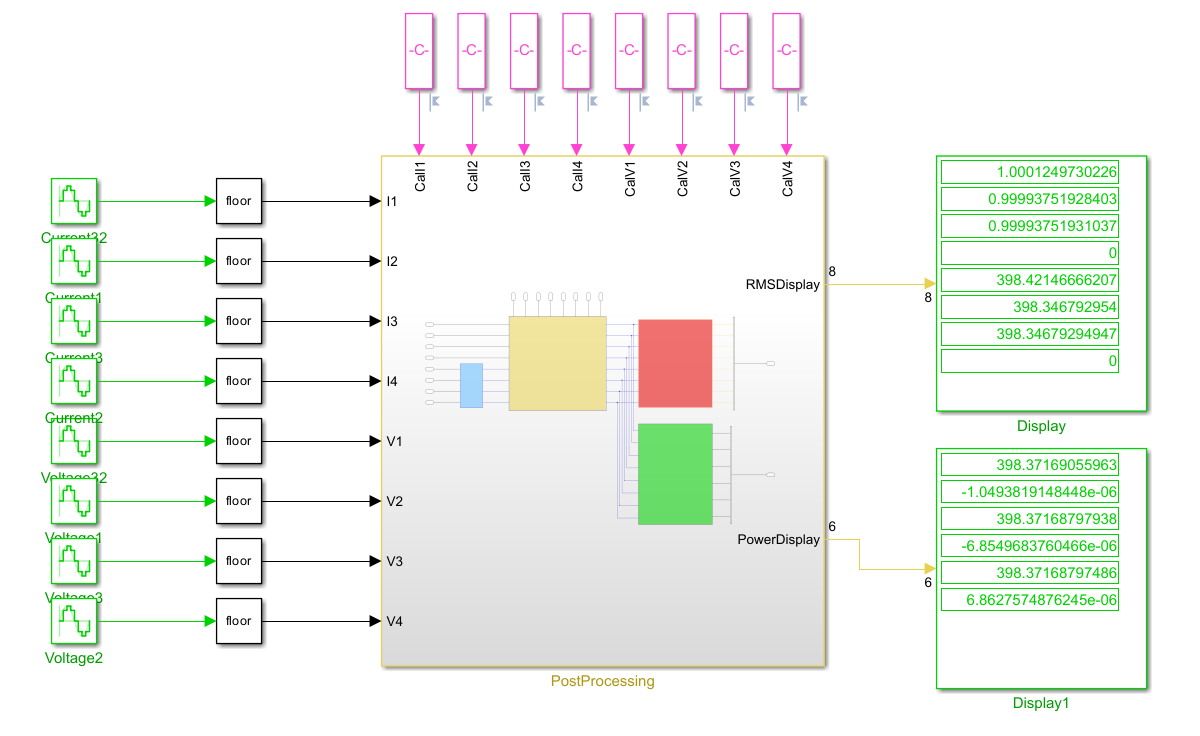
\includegraphics[scale=0.33]{images/Feature Extraction.png}
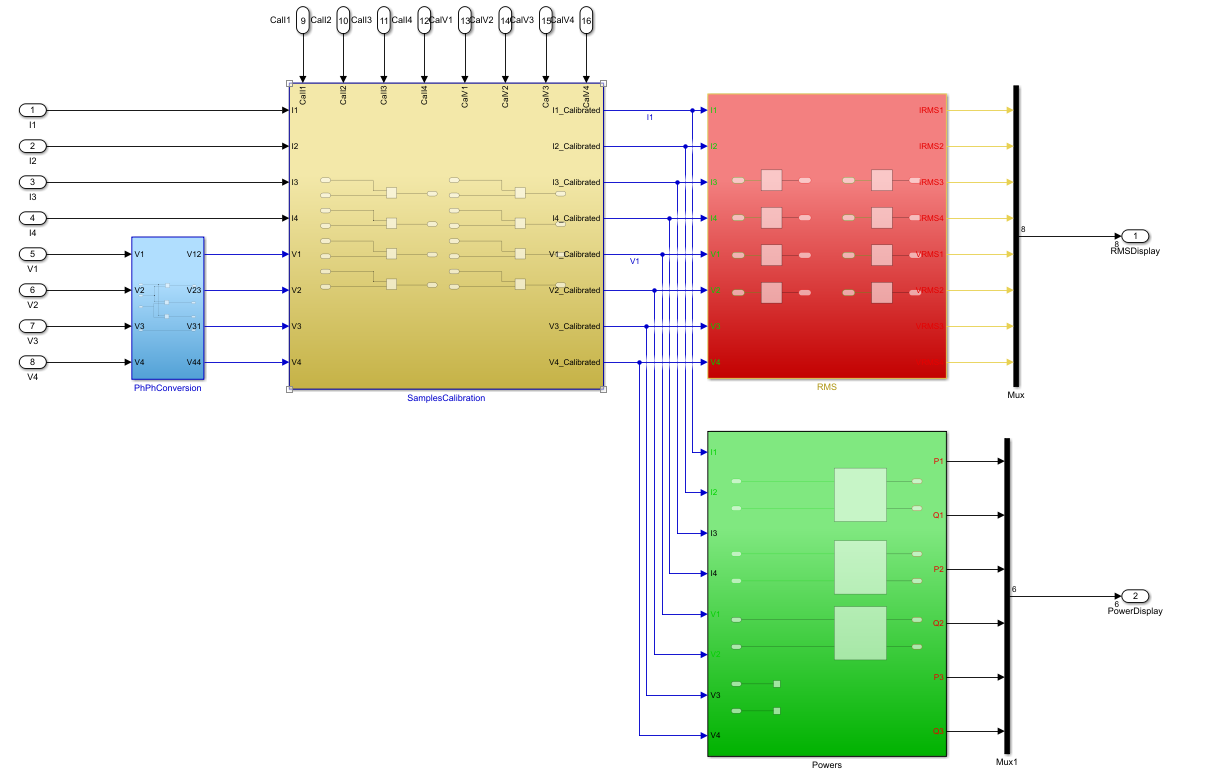
\includegraphics[scale=0.33]{images/PostProcessing.png}
\caption{Embedded Algorithm for Acquisition System}
\label{fig:x Embedded Algorithm}
\end{figure}

In the figure \ref{fig:x Embedded Algorithm}, we have designed an embedded algorithm in simulink to serve the RMS calculation purpose for our acquisition system.In the left block, there are 8 distinct analog signals originating from 8 channels of the ADS131M08. Additionally, 8 unique calibration factors are directed towards the \textbf{PostProcessing } block. The \textbf{RMSDisplay} and \textbf{PowerDisplay} blocks depict the computed outcomes during simulation. On the right block, the PostProcessing segment has been constructed, within which a \textbf{PhPhConversion} block (depicted as Blue) is utilized to analyze the three-phase voltages. The variance across two lines as the phases intersect at an angle is commonly termed as the line-to-line voltage. In the PhPhConversion block, the calculation of the differences between V1, V2, and V3 is carried out, with V4 representing the ground reference.
In the \textbf{SamplesCalibration} block (depicted as Yellow), all these analog signals undergo calibration using the 8 distinct calibration factors. Subsequently, the RMS is determined by the Red Block, while the Power values are computed by the Green Block.\par
\vspace{0.5cm}

In Figure \ref{fig:x Cal_RMS Block }, the left illustration represents our \textbf{SamplesCalibration} process, wherein every individual sample is divided by its corresponding calibration factor. Meanwhile, the right depiction showcases the application of the \textbf{Moving RMS} block. This block computes the moving RMS of the input signal for each channel independently over a specific time duration. The block squares the data samples, multiplies them by a series of weighting factors, and then adds the weighed data in the exponential weighting process. The RMS is then calculated by the block by calculating the sum's square root.\par

\begin{figure}[htbp]
\centering
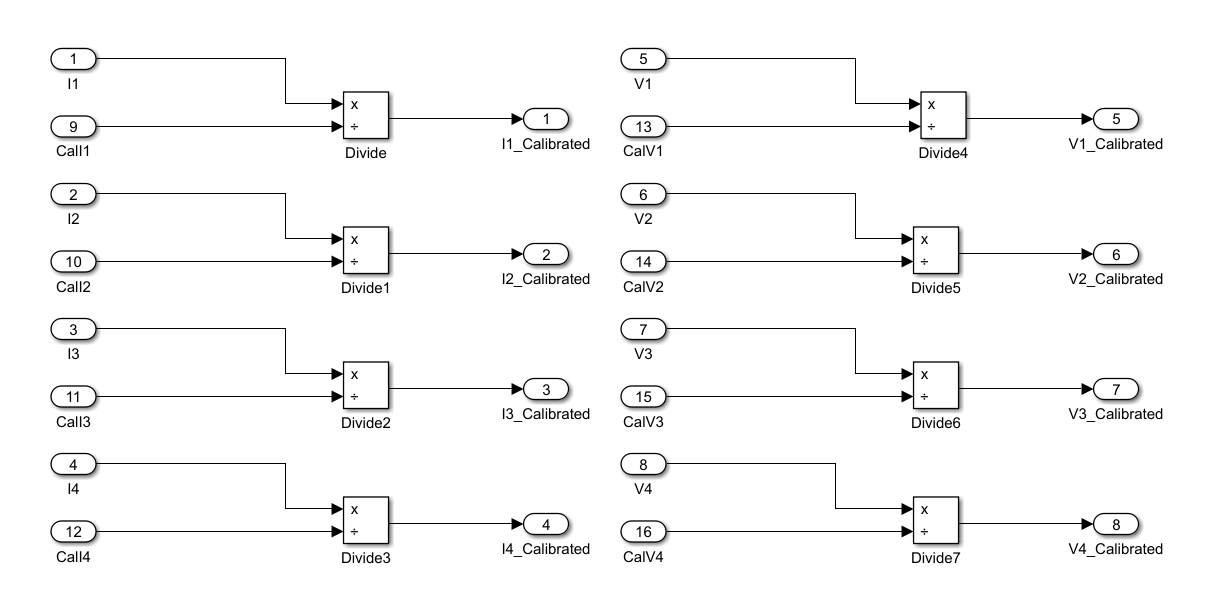
\includegraphics[scale=0.4]{images/Sample_Calibration.PNG}
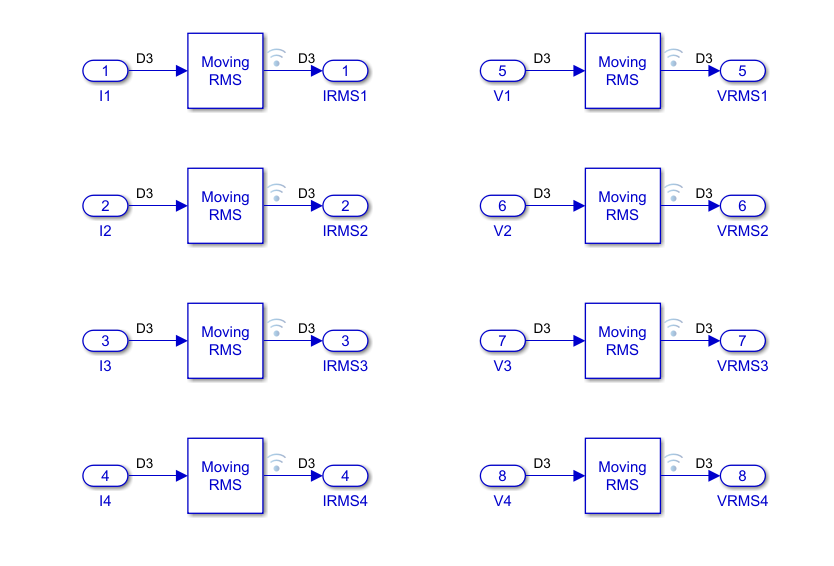
\includegraphics[scale=0.4]{images/RMS.png}
\caption{Calibration and RMS Calculation Block}
\label{fig:x Cal_RMS Block }
\end{figure}

\textbf{Simulink Embedded Coder:}
We can create effective, condensed, and optimized C and C++ code from our Simulink models and Stateflow diagrams using this robust tool from MathWorks. In particular for embedded systems and real-time applications, it is a crucial part of the MathWorks ecosystem. We can automatically create code for a range of hardware targets, including microcontrollers, CPUs, and FPGAs, thanks to Simulink Embedded Coder.


 \begin{figure}[htbp]
\centering
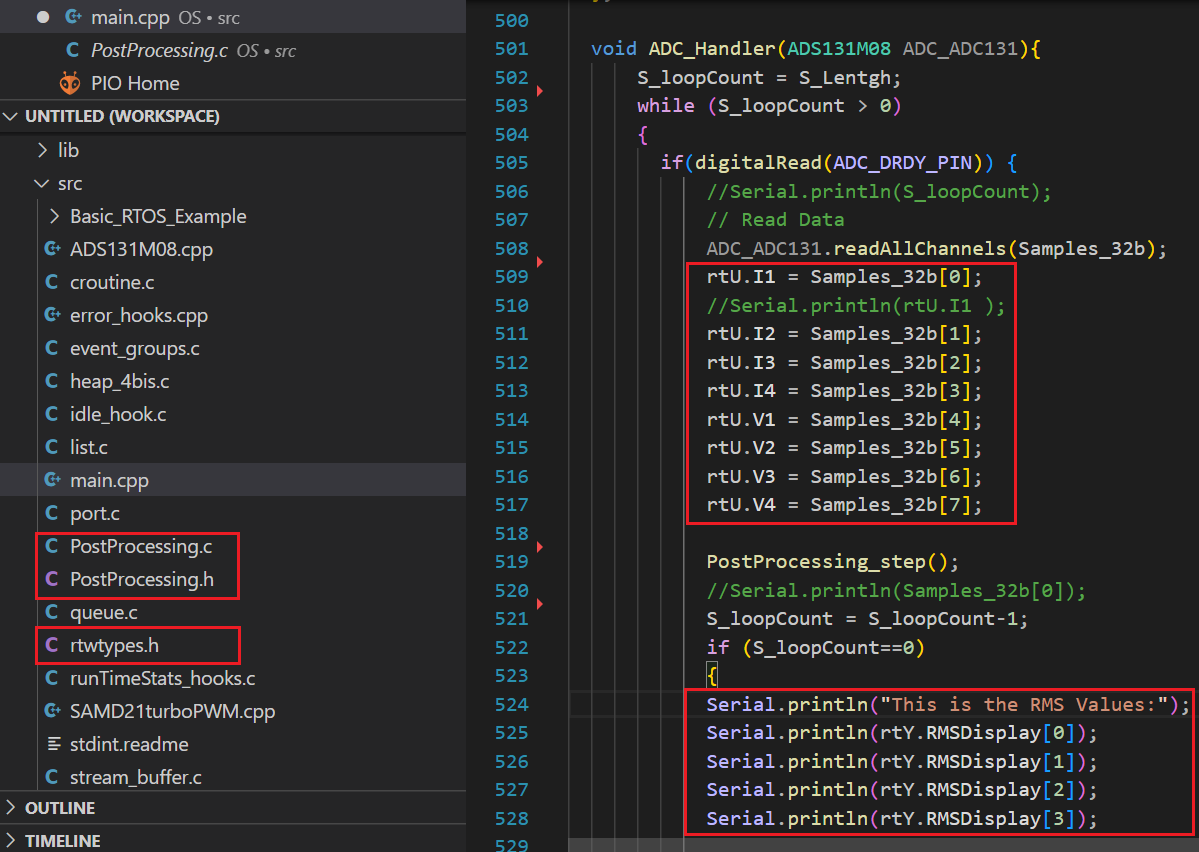
\includegraphics[scale=0.6]{images/RMS Calculation.PNG}
\caption{Utilyzing Simulink generated code in our firmware}
\label{fig:x Algorithm RMS}
\end{figure}

We have generated C code of PostProcessing block from our designed algorithm.Three generated files \textbf{‘PostProcessing.c’},\textbf{‘PostProcessing.h’}, and \textbf{‘rtwtypes.h’} has been added to the firmware shown in figure \ref{fig:x Algorithm RMS}. The purpose of rtwtypes.h is to define platform-independent data types that ensure consistent data representation across different target platforms. These data types are used in the generated code to ensure that the behavior of the Simulink model is preserved when running on different hardware. \textbf{rtU.I} represents the 32 bit analog current samples, and \textbf{rtU.V} represents the voltage samples. The function \textbf{PostProcessing\_step()} runs our designed algorithm for these sample data calculation. Then \textbf{rtY.RMSDisplay} is the output which will be displayed in our serial monitor. We have tested the RMS for the 1st channel by supplying 1amp current to the ADC, and this Simulink Algorithm represented 0.991 amp in serial monitor after calculation.

\nomenclature{$IDE$}{Integrated Development Environment}
\nomenclature{$RTOS$}{Real Time Operating System}
\nomenclature{$CRC$}{Cyclic Redundancy Check}
\nomenclature{$OSR$}{Oversampling Ratio }
\nomenclature{$HTTP$}{Hypertext Transfer Protocol}
\nomenclature{$DSP$}{Digital Signal Processors}
\nomenclature{$ASIC$}{Application-specific Integrated Circuits}
\nomenclature{$FPGA$}{Field-programmable Gate Arrays}



